\chapter{Literature Survey}
\label{ch:quadcopter}
In this chapter we will familiarize with quadcopter, its components and
technical specifications. We will also discuss the prior work related to
mainly three areas: control and navigation of quadcopter, mosaicing, and
fiducial based tracking . 
\section{Quadcopter}
The necessity for flying device with greater maneuverability and hovering
ability led to creation of a quadcopter. A quadrocopter or quadcopter  is a
multirotor helicopter that is lifted and propelled by four rotors. The
four-rotor design allows quadcopters to be relatively simple in design yet
highly reliable and maneuverable. Quadcopter  is a  symmetrical vehicle which
has four rods with propellers connected to rotors  at each end. Two diagonally
opposite propellers rotate in clockwise(CW) direction while remaining  two
rotate in counterclockwise(CCW) direction as shown in
Figure~\ref{fig:quadcopter}(Middle). This is done in order to balance the
torque generated by each pair of rotors. The angular movement (roll-pitch-yaw)
around three axes coordinate system of quadcopter is shown in
Figure~\ref{fig:quadcopter}(Right).


\begin{figure}[b!]
  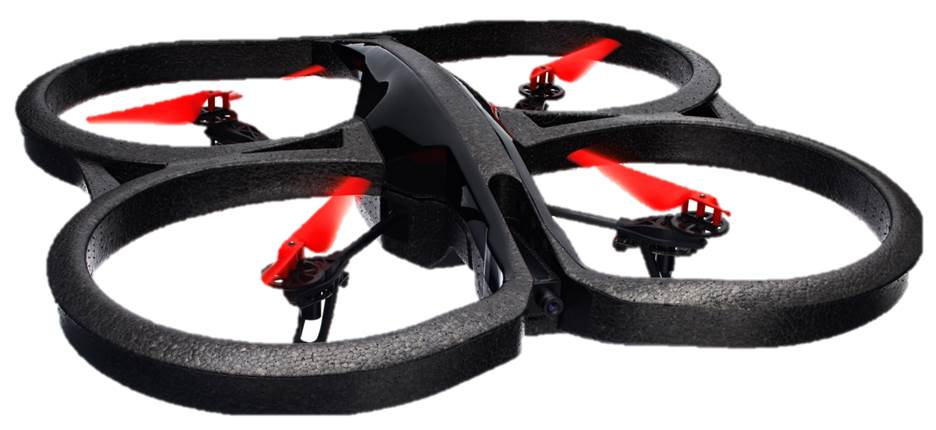
\includegraphics[width=0.3\linewidth]{images/ardrone2}	
  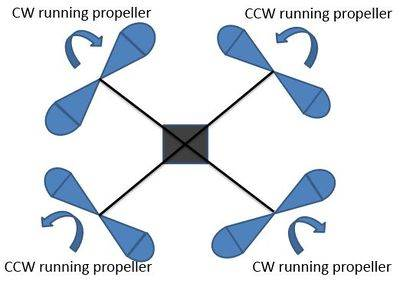
\includegraphics[width=0.34\linewidth]{images/quadrotor}
  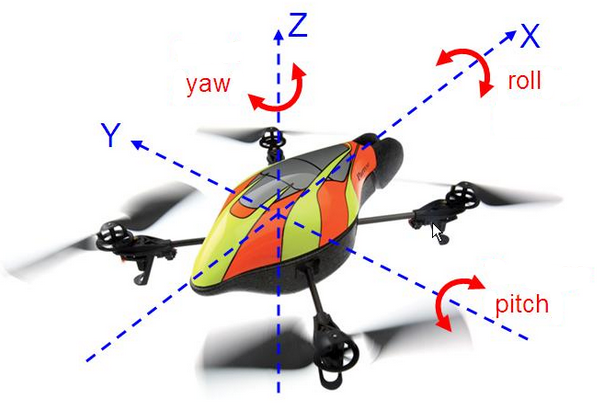
\includegraphics[width=0.34\linewidth]{images/rpy}
  \caption[Quadcopter Motions]{Left: Sample quadcopter, Parrot's ARDrone 2.0.
  Middle: Direction of propeller movement of quadcopter. Right: Rotation of
  quadcopter along three axes. [Picture Courtesy: Google image search]}
  \label{fig:quadcopter}
\end{figure}

The speed of each rotor can be independently varied through onboard flight
controller to achieve various controls. For example, if we would like to hover
the quadcopter, the thrust generated by all rotors should match the weight of the
quadcopter. If we want to move in any direction, then controller tilts the
quadcopter on that side by increasing speed of rotors on other side. The
horizontal component of the thrust will move the quadcopter in that direction.
If we want to rotate the quadcopter around z-axis, i.e., to change its yaw,
controller imbalances the torque purposefully by increasing speed of rotors on
one diagonal. For e.g., if we increase speed of rotors which are rotating in
clockwise direction, quadcopter will turn in counterclockwise direction.
This is illustrated in Figure~\ref{fig:quadcopterMotion}.

\begin{figure}[h!]
  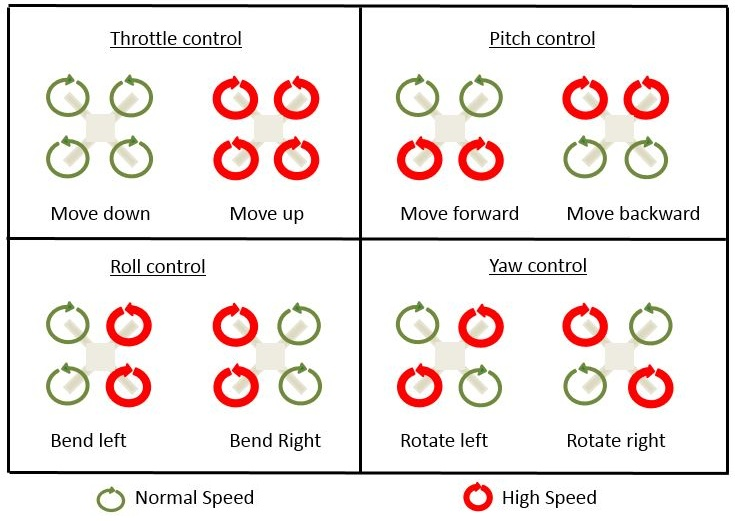
\includegraphics[width=\textwidth]{images/quadcopterMotion.jpg}
  \caption[Speed control of rotors for quadcopter's motion]{Speed control of
  rotors for quadcopter's motion.
  (Left-Top): Speed of all rotors is increased/decreased to move
  quadcopter up/down.
  (Right-Top): To move quadcopter in forward/backward direction, we increase
  speed of rear/front rotors.
  (Left-Bottom): To move quadcopter in left/right direction, we increase
  speed of right/left rotors.
  (Right-bottom): To rotate quadcopter in clockwise direction, we increase speed
  of rotors moving in counterclockwise direction and vice-versa. 
   [Picture Courtesy: Google image search]}
  \label{fig:quadcopterMotion}	
\end{figure}

Quadcopter mainly contains three subsystems: Inertial Measurement Unit (IMU),
Imaging system, and Communication system all connected to Central Processing
Unit, an ARM processor. IMU is responsible for getting the pose of quadcopter.
Imaging system deals with capture and storage of images of surrounding
environment. Communication system handles interfacing between quadcopter and
client device. Here, we have given details of Parrot's AR Drone 2.0 as we are
using the same for our experiments. Though components will remain mostly same across
different quadcopters, technical specifications (e.g., image resolution) may
vary across various models.

\subsection{Inertial Measurement Unit (IMU)}
Every quadcopter has Inertial Measurement Unit (IMU) onboard in order to maneuver
quadcopter in controlled way. IMU is an electronic device which measures forces
acted upon the body of quadcopter. It comprises of 3-axis accelerometer, 3-axis
gyroscope, 3-axis magnetometer, and ultrasound altimeter (also called as sonar).
Accelerometer measures acceleration of quadcopter along 3 axes while gyroscopes
measures angular movement around 3 axes, i.e., roll, pitch and yaw. Magnetometer
measures angular movement with respect to magnetic axis of earth, to get
absolute angle from magnetic axis. Sonar measures quadcopter's
height from the ground.

Sometimes IMU also have pressure sensor to measure the air-pressure around the
device. It is helpful in checking if there is a strong wind so that
onboard flight controller can take the corrective action to stabilize the
quadcopter. 

IMU provides us information about linear as well as angular accelerations. This
information is later used to estimate the pose of the quadcopter. However, due
to various factors such as noisy measurements, environmental disturbances, the
estimated pose may be completely off.
 
\subsection{Imaging System}
Parrot's ARDrone 2.0 has two cameras, front camera with a wideangle lens
($92^{\circ}$ diagonal) to capture images with HD resolution (1280 $\times$ 720
pixels) at 30 FPS, while vertical camera (pointing downwards) having QVGA
resolution (320 $\times$ 240) at 60 FPS used for measuring ground speed.
Though front camera can capture the images at HD resolution, it can transmit
images over Wi-Fi at only  lower resolution (640 $\times$ 360 pixels). Hence we
need to use USB storage device on quadcopter to store a video streamed by the
quadcopter camera. 

\subsection{Communication System}
The AR.Drone 2.0 can be controlled from any client device supporting WiFi. The 
process followed is :
\begin{enumerate}
  \item The AR.Drone creates a WiFi network with an SSID usually named
adrone2\_xxx (where xxx is manufacture date in YYYYMMDD format) and self
allocates a free, odd IP address (typically 192.168.1.1).

   \item The user connects the client device to this SSID network.
   \item The client device requests an IP address from the drone DHCP server.
   \item The AR.Drone DHCP server grants the client with an IP address which is
   the drone's own IP address plus a number between 1 and 4 e.g., 192.168.1.3
   \item The client device can start sending requests (Land, Takeoff, etc.) to
   the AR.Drone IP address and its services ports
\end{enumerate}

ARDrone 2.0 can be controlled from client device through 3 main communication
services: 
\begin{itemize}
\item \textit{AT} commands for control and configuration are sent on UDP
port 5556.
\item Information about the drone (like its status, position,  speed, 
etc.), called as \textit{navdata}, is sent by the drone to its client on UDP
port 5554.  
\item A video stream is sent by the AR.Drone to the client device on UDP port
5555.
\end{itemize}

Now, we will see prior work done in the field of quadcopter navigation,
mosaicing of scenes, and tracking of quadcopter.

\section{Control and Navigation of quadcopter}
In this section we will discuss manual as well as autonomous ways to navigate
a quadcopter, specifically Parrot's ARDrone 2.0.
Parrot has released an mobile app, AR.FreeFlight on iPhone as well as Android
phones for piloting ARDrone. This App can be used to do simple maneuvers such
as going left/right, forward/backward, up/down. It also has a ``Director mode'',
which allows some advanced maneuvers such as circling around itself to take
panoramic view. But still it is very difficult to maneuver the drone without
expertise.

\begin{figure}[h!]
  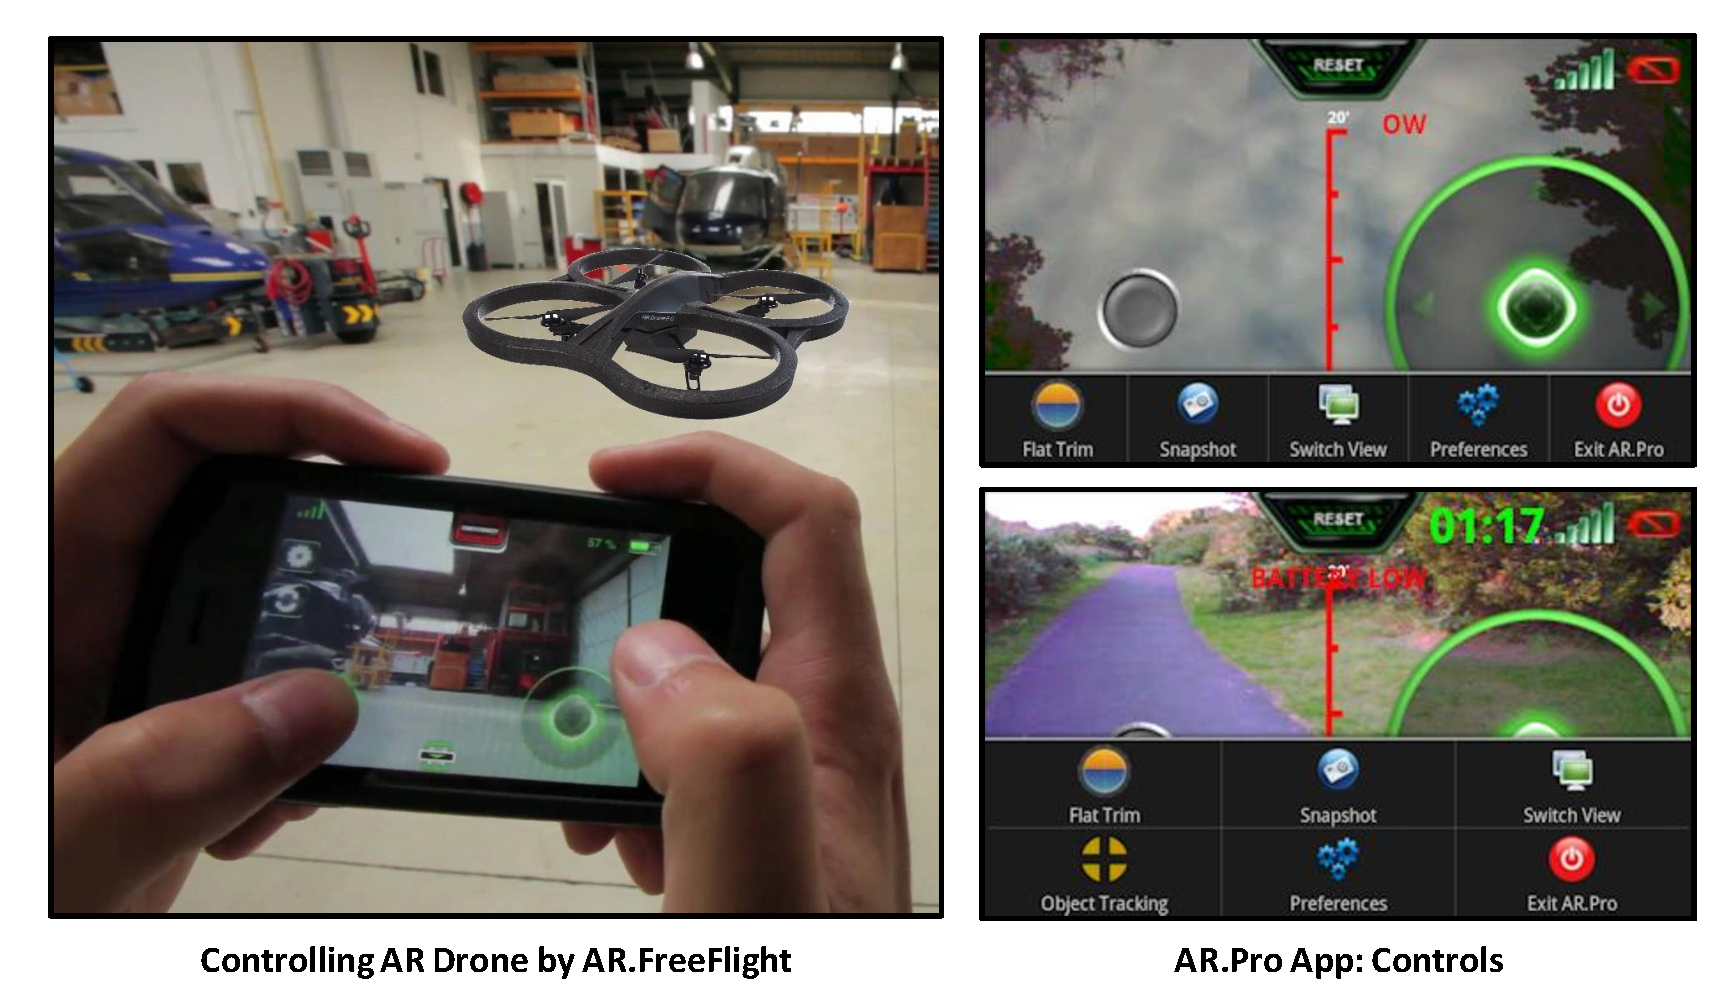
\includegraphics[width=\textwidth]{figures/manualControl}
   \caption[Manual control of Parrot's ARDrone 2.0]{Manual control of Parrot's
  ARDrone 2.0 through smartphone. Left: Parrot's AR.FreeFlight is used to
  control the ARDrone 2.0. 
  Right: Alternatively one may use AR.Pro having advanced features for control.
  [Picture Courtesy: Google image search]}
   \label{fig:manualControl}
\end{figure}

There are also some paid apps such AR.pro for piloting AR Drone. AR.pro app
have some advanced settings which are not available in AR.Freeflight e.g.,
changing WiFi channel, Altitude limiter, Dual Joystick support, etc. All of
these apps as well as softwares have main limitation that as it involves lot of manual
intervention, it lacks precision, which is required in imaging application.
E.g., if we want quadcopter to complete a rectangular loop and come back to its original
position, it fails to do so. 

Some flight controller softwares use add-on GPS for autonomous navigation of
quadcopter. However in GPS denied areas e.g., indoor, we can not use such
softwares. Even in outdoor, we cannot rely on only GPS for accurate
navigation of quadcopter due to issues like spurious GPS signals, GPS jammers,
etc.

Another way to accurately navigate quadcopter is to use techniques such as
Simultaneous Localization And Mapping(SLAM)\cite{Davison:2007} or Parallel Tracking And
Mapping(PTAM)\cite{klein}. SLAM or PTAM algorithm first builds a 3D map of
surrounding environment and then estimates device's current position.

Engel et al.~\cite{Engel12} have developed a method for navigation of quadcopter
based on PTAM\cite{klein}. Engel et al. have used Extended Kalman Filter (EKF)
to fuse visual observation model with the odometry observation model to estimate
the pose of the quadcopter. They have also developed a method for
correctly estimating scale of the built 3D map. But, they have not ensured
a hundred percent scale accuracy which results in an inaccurate 3D map of
the surrounding environment.

\section{Mosaicing of scenes}
Panoramic image stitching (alternatively, image mosaicing) is a
well-studied problem in the field of computer vision.  Representative
works include~\cite{Milgram1975}, \cite{Milgram1977}, \cite{Capel},
\cite{Szeliski1997}, \cite{Brown07}, \cite{Brown03}.  A full discussion
on related works is outside the scope of this work, readers are
referred to~\cite{Szeliski05imagealignment} for an excellent survey.
Given the maturity of this area, there are various freeware as well as
commercial software available for performing image stitching; most
notable are AutoStitch \cite{autostitch}, Microsoft\textsc{\char"13}s Image
Compositing Editor \cite{ICE}, and Adobe\textsc{\char"13}s Photoshop
\cite{photoshop}.

All of these methods are based on a similar strategy of finding
features in each image, matching these features between images, and
then computing pairwise image warps to align them together.  A 
bundle adjustment is often applied to globally refine the alignment.
All of the aforementioned methods assume the imaged scene is planar or
that the camera has been rotated carefully around its center of
projection to avoid parallax.

Brown \etal \cite{Brown05} have used a new type of invariant features
located at Harris corners in discrete scale-space and oriented using a
blurred local gradient for stitching. Eden \etal \cite{Eden} were
able to stitch images with large exposure difference as well as large
scene motion into single HDR quality image without using any
additional camera hardware.

All of the image mosaicing methods work only when there is an
``intersection'' in feature space of images to be stitched. When there
are ``gaps'' (either physical or due to lack of features) between
images to be stitched it is not clear how to perform the
stitching. Structure from Motion methods also rely on overlap of
features and fail when images have gaps. In this work, we discuss how
to use the available IMU data that accompanies our input images to
help overcome these problems.

\subsection{Mosaicing of Aerial Imagery}
TODO. [MGP: I am unable to get 'good' papers on this topic, any suggestions.
Basically I would like to contrast our work with other mosaicing work done on
aerial images.]

\section{Fiducial Markers and Tracking}
Inexpensive quadcopter such as Parrot's AR Drone have very jerky movement. Hence,
it is difficult to track the objects through quadcopter or even the quadcopter
itself. In this section we will review the prior work done related to the
tracking aspect of the quadcopter.\\

\noindent\textbf{Fiducials:}~Fiducials are often used to evaluate the planning
algorithms given that ground truth positions can be detected by the
quadcopter's camera. Figure~\ref{fig:previous_work} shows a few
examples of existing fiducials.  Many designs use a two
dimensional barcode inside a rectangular grid. One example of such a
fiducial is from the ARToolkit~\cite{ARToolkit02}, a well known
toolkit used in many augmented reality (AR) applications. Kato and
Billinghurst~\cite{kato-artoolkit} first demonstrated the use of
ARToolkit in various augmented-reality-based applications.

\begin{figure}[b!]
\centering
 \begin{subfigure}[b]{0.29\linewidth}
  \centering
  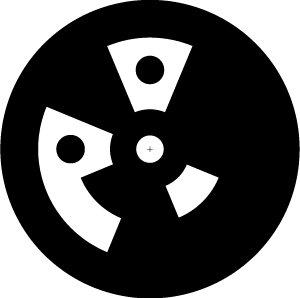
\includegraphics[width=0.8\linewidth]{figures/fiducial/intersense.jpg}
  Circular Data Matrix~\cite{NaimarkF02}
 \end{subfigure}\quad
 \begin{subfigure}[b]{0.2\linewidth}
 \centering
  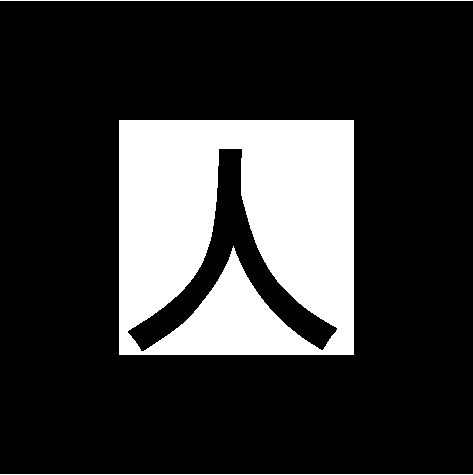
\includegraphics[width=\linewidth]{figures/fiducial/pattKanji.pdf}
  ARToolkit~\cite{ARToolkit02}
 \end{subfigure}\quad
 \begin{subfigure}[b]{0.2\linewidth}
  \centering
  
\includegraphics[width=\linewidth]{figures/fiducial/ARtag.jpg}
  ARTag\quad~\cite{Fiala05}
 \end{subfigure}\quad
 \begin{subfigure}[b]{0.2\linewidth}
  \centering
  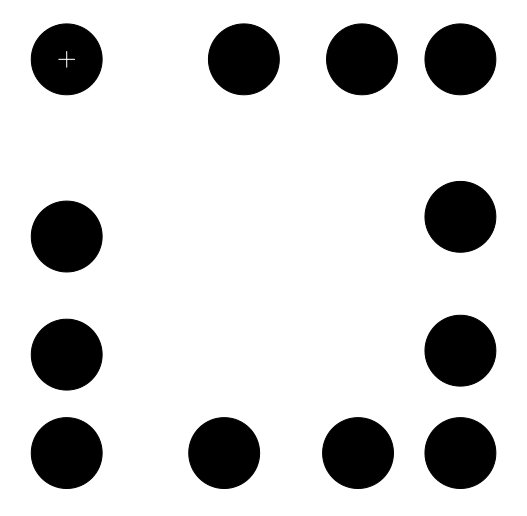
\includegraphics[width=\linewidth]{figures/fiducial/pifiducial.jpg}
  PiTag\quad~\cite{Pitag13}
 \end{subfigure}
 %\quad
%  \begin{subfigure}[b]{0.14\linewidth}
%   \centering
%   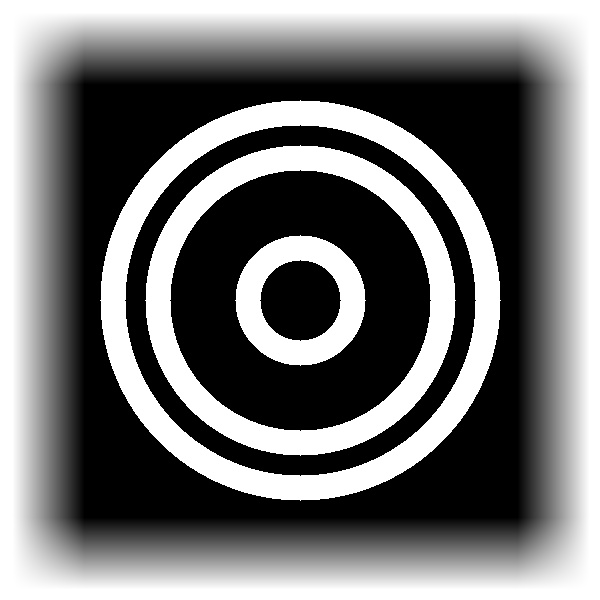
\includegraphics[width=\linewidth]{figures/fiducial/our_fiducial.jpg}
%   Our Fiducial
%  \end{subfigure}
 \caption[Prior fiducials]{Prior fiducials and our proposal. 
 While each code has its pros and cons depending on the environment, no
 prior code is expressly designed to be recognized under motion blur.}
 \label{fig:previous_work}
\end{figure}


Fiala~\cite{Fiala05} proposed a fiducial termed, ARTag, which is a
bi-tonal system consisting of a square border and an interior
6$\times$6 grid of black or white cells. The improvement of the ARTag
compared to the ARToolkit lies in the detection of corners instead of
detection of lines to find possible patterns.  This proved to be more
efficient than \cite{ARToolkit02} in terms of recognition rate as well
as the number of different patterns which can be created.  {\it The
reliance on both line and corner detection, however, hampers
recognition under motion blur.}

There were also attempts to use circular patterns instead of
rectangular.  Gatrell et al.~\cite{concentric} used concentric circles
for monocular pose estimation as well as object identification. Cho et
al.~\cite{Cho:2001,Cho97fastcolor} have used multicolor rings instead
of black and white rings~\cite{concentric} to increase possible number
of fiducials.  These multicolor rings are used in wide area tracking
in large scale applications.  {\it Although based on  concentric rings, these
approaches require the complete ring to be recognized; this is
impractical when the pattern undergoes directional motion blur.}

Naimark and Foxlin~\cite{NaimarkF02} proposed a circular bar code
called the Circular Data Matrix that is beneficial in terms of easy
detection and ability to have a large number of uniquely identifiable
codes.  To address the issue of occlusion, Bergamasco et
al.~\cite{runetag11} proposed the RUNE-tag fiducial by creating a
number of circular dots arranged in circular fashion. RUNE-tags can be
detected even when 50\% of the fiducial area is occluded. Bergamasco
et al.~\cite{Pitag13} proposed the PiTag fiducial, also composed of
circular structures but arranged in a rectangle, to exploit projective
invariant cross-ratio.  This provided similar occlusion resistance as
RUNE-tag but with even less circular dots. {\it All of these techniques,
however, rely on generic feature detection (e.g., circle detection)
and such algorithms break down under motion blur.}\\

%Zhang et al.\cite{Zhang:2002} and Claus et al. \cite{ClausF04} have done
%quite comprehensive comparative study of various fiducial systems with
%respect to processing time, recognition rate and accuracy with
%respect to viewing angle and distance.

\noindent{\textbf{Tracking:}}~~Fiducial detection between successive video
frames can be considered as a tracking problem where the tracked
object is the fiducial.  There is a very large body of research
dedicated to tracking and interested readers are referred
to~\cite{Yilmaz:2006} for a good survey.

Most tracking methods~\cite{Ross:2008,Wu:2009,Perez02,Mei:2009} assume
the image sequence to be blur free. In reality, however, the presence
of motion blur in a video sequence is often unavoidable. To this end,
Wu et al.~\cite{Wu:2011} proposed the Blur-driven Tracker (BLUT)
framework for tracking motion-blurred targets. BLUT is based on the
observation that although motion blur degrades the visual features of
the target, it may also provide useful cues about the movements to
help tracking.

The BLUT framework successfully tracks a blurred target when there is
uniform motion, and the position of the tracked object does not change
drastically in successive frames. However, the erratic motion from the
quadcopters, as well as the problem of dropped video frames makes the task too
problematic for BLUT to successfully track.

In this chapter, we got acquainted with quadcopter, motion control, its
components. We also have seen limitations of existing methods for quadcopter
travel and imaging.  We will discuss how these limitations are addressed in
upcoming chapters.